\chapter{The \cherimcuisa{}}
\label{chap:cheri-riscv}


\newcommand{\riscvloadcappagefault}{0x1A}
\newcommand{\riscvstorecappagefault}{0x1B}
\newcommand{\riscvcheriexception}{0x1C}
\newcommand{\caprootX}{$\top_{X}$}
\newcommand{\caprootM}{$\top_{M}$}
\newcommand{\caprootS}{$\top_{S}$}

The \cherimcuisa{} extends RV32~\cite{RISCV:User:2.2} with CHERI~\cite{UCAM-CL-TR-951} memory safety features.
It is designed to be a very minimal subset of RISC-V and CHERI that supports strong spatial and temporal memory safety, and compartmentalization.
This is intended to be a concise description of the architecture and currently assumes some familiarity with both CHERI and RISC-V.

\section{Starting subset of RV32}

The \cherimcuisa{} is based on a minimal subset of RV32 supporting machine mode only (i.e. no virtual memory).
The C instruction compression extension is required (with minor modifications) and always enabled in the \asm{misa} CSR.
PMP support is optional, although we anticipate that it will not add value owing to the strong protections already offered by the \cherimcu{} ISA and RTOS combination.
Floating point is optional and may conflict with some encoding choices for compressed instructions.

\section{Omitted CHERI features}

Those familiar with CHERI-RISC-V will note that some features are omitted to simplify the architecture at the cost of a little flexibility and backwards compatibility.
In particular, CHERI hybrid mode is not supported, so there is no need for \DDC{} or a cap mode bit in \PCC{}.
Instead all code runs in pure-cap mode, where existing instructions use capabilities for address operands.
Offset addressing is also eliminated, so the \insnnoref{CGetOffset} and \insnnoref{CSetOffset} instructions are not present and special capabilities registers (including \PCC{}) are always interpreted simply as their address, rather than as an offset relative to the base as in CHERI-RISC-V.
This allows us to drop checks for the alignment of the base of executable capabilities as there is no possibility of confusion arising from an unaligned base, as there is in hybrid mode CHERI-RISC-V.

\section{Changes to register file}

The 16 32-bit integer registers from RV32 are extended into 65-bit \emph{capabilities} (64-bits $+$ tag).
Abstractly, capabilities have the following fields:
\begin{description}
  \item[address] A 32-bit address or integer value.
  \item[base] The 32-bit inclusive lower bound.
  \item[top] The 32-bit exclusive upper bound.
  \item[perms] The capability permissions (\cref{sec:perms}).
  \item[otype] Used for sealing (\cref{sec:sealing}).
  \item[tag] A single bit indicating valid or invalid.
  Capabilities with this bit set are called \emph{tagged}.
\end{description}
The actual capability encoding is compressed as described in \cref{sec:capenc}.
Instructions that read integer operands use only the lower 32-bits (the capability \caddress{}).
Instructions that produce integers write a NULL capability (\cref{sec:null}) with the \caddress{} set to the integer result.
In assembly the capability registers are referred to as \asm{\$c0..\$c15}, with \asm{$x0..$x15} referring to their address parts.
At reset the registers are initialized to the NULL capability.

\section{Instruction encodings}

As described in \cref{app:isaquick-riscv} the new capability instructions use major opcode 0x5b and the standard I-type and R-type formats.
Additionally \insnriscvref{AUICGP} uses major opcode 0x7b.

\section{Changes to instruction fetch / control flow}

The program counter is extended to a capability, \PCC{}, with \PCC{}.\caddress{} assuming the role of the \PC{}.
If \PCC{} becomes untagged or the instruction is not entirely within the bounds of \PCC{}, then an exception is raised.
Note that the bounds check must take account of whether the fetched instruction is 2 or 4 bytes.
If the program counter is outside the bounds of \PCC{} it might be unrepresentable in the compressed capability format (\cref{sec:bounds,sec:repcheck}).
Therefore, to avoid violating capability monotonicity the value written to \MEPCC{} when there is an instruction fetch bounds violation has its tag cleared.
Due to unrepresentability the bounds of \MEPCC{} might not correspond to the bounds of \PCC{} at the time of the exception in this case.

\insnriscvref{CJALR} replaces the \asm{JALR} instruction and uses capabilities for the target and link register.
It checks that the target capability is tagged and executable before it is installed in \PCC{}.
If the target is sealed with one of the reserved `sentry' types then it is unsealed before jumping to it, while possibly writing \asm{mstatus.MIE} (see \cref{sec:sealing}).
If it is sealed with a non-sentry type an exception is raised.

The link register written by \insnriscvref{CJAL} and \insnref{CJALR} is sealed as a sentry of the type corresponding to the current value of \asm{mstatus.MIE}.

The checks on \insnriscvref{CJALR} and special capability writes (\cref{sec:scrs}) prevent execution with a \PCC{} that is sealed or lacks \cappermX{}.
The only ways for \PCC{} to become untagged is by \asm{MRET} with an untagged \MEPCC{} or exception with untagged \MTCC{}.
The latter will result in an unrecoverable exception loop.

\section{Changes to memory accesses}

All existing load and store instructions are modified to take a capability for the base address.
The address of the capability is used as the base address for the memory operation and an exception is raised if the capability:

\begin{itemize}
  \item has the tag unset
  \item is sealed
  \item does not have the appropriate memory permissions (\cref{sec:perms})
  \item has bounds that do not cover the entire region being accessed
  % \item TODO color check?
\end{itemize}

\section{Tagged memory}

Memory is extended with a single tag bit for each capability sized and aligned memory location.
The new capability load and store instructions, \insnriscvref{CLC} and \insnriscvref{CSC}, transfer a capability-sized-and-aligned region of memory to or from a register, including the tag bit.
The tag bits are not accessible directly and may be set to one only by a store of a tagged capability using \insnriscvref{CSC}.
To prevent tampering with valid capabilities in memory, non-capability stores (e.g. \asm{CSW}) clear the tag bits for the capability-aligned region(s) they touch.
If an unaligned store crosses a capability alignment boundary then two tag bits need to be cleared.

The platform must define which regions of memory support capability tags.
In memory without tag support capability stores will silently drop the tag, and capability loads will always return untagged values.
The value of the tag bits is undefined at reset, so software should take care to zero all memory on start up unless running on a platform that defines them to be zero.

\section{Temporal safety}
\label{sec:temporal}

In addition to the capability tag bits there is a revocation bit for each \emph{revocation granule} (currently the same size as a capability, 8 bytes).
After loading a capability with the tag set, the \insnriscvref{CLC} instruction loads the revocation bit corresponding to the \cbase{} address of the capability (N.B. not the \caddress{}).
If the granule's revocation bit is set then the capability's tag is cleared before writing it to the destination register.
The revocation bits are memory mapped so that they can be manipulated by the allocator.
The platform defines the location of revocation bits in the address space and their mapping to addresses.
Not all mapped addresses need have corresponding revocation bits:
capabilities whose \cbase{} points to a region of address space without corresponding revocation bits will not be revoked by \asm{CLC}.
It is the responsibility of software to allocate capabilities in regions with revocation bits when support for revocation is desired.

A typical implementation is expected to exclude all of the MMIO space from the revocation bitmap.
In addition, an implementation with multiple SRAM banks may support revocation only for some granules.
Memory used for code and globals will never be revoked (in the software model) and so may be excluded.
An implementation may also provide a configuration interface that allows software to specify the range of heap memory and avoid the cost of the load barrier on globals.

The \cbase{} of sealing capabilities (see \cref{fig:compressedperms}) refers to a distinct namespace to that of memory capabilities, therefore they are not revoked using this mechanism.
Software should take care not to reallocate sealing capabilities unless there is some other mechanism to revoke previously issued ones.
Given the $2^{32}$ sized space for sealing capabilities we expect most applications will never have to reallocate them.

Like the capability tag bits, the value of the revocation bits in memory is undefined on reset unless defined by the platform.

\section{Controlling access to system registers}
\label{sec:asr}

In the absence of supervisor or user modes, it is useful to be able to restrict access to sensitive control and status registers (CSRs) and special capability registers (SCRs).
The \cappermASR{} permission on executable capabilities can be used to enable or disable access to certain special registers.
If \cappermASR{} is set on the current \PCC{} then access to all registers is permitted, otherwise attempting to access restricted registers or execute \insnnoref{MRET} will cause a \cappermASR{} exception.
\cref{tab:risc-v-access-system-registers-whitelist} shows the allowlist of CSRs that can be accessed without \cappermASR{}.
Similarly \cref{tab:risc-v-special-capability-registers} lists the access requirements for special capability registers.

\begin{table}[h!]
\centering
\begin{tabular}{cc}
\toprule
\textbf{CSR}           & \textbf{Read/Write} \\
\texttt{cycle(h)}      & Read-Only           \\
\texttt{time(h)}       & Read-Only           \\
\texttt{instret(h)}    & Read-Only           \\
\texttt{hmpcounter(h)} & Read-Only           \\
[1.5em]
\texttt{fflags}        & Read-Write          \\
\texttt{frm}           & Read-Write          \\
\texttt{fcsr}          & Read-Write          \\
\bottomrule
\end{tabular}
\caption{CSR allowlist. The accesses shown are the only CSR accesses that are permitted when the installed PCC does not have the \cappermASR{} permission bit set.}
\label{tab:risc-v-access-system-registers-whitelist}
\end{table}

\section{Special capability registers}

\label{subsection:cheri-riscv-scrs}
\label{sec:scrs}

Special Capability Registers (SCRs) are similar to RISC-V's Control and Status Registers (CSRs) except that they contain capabilities rather than integers.
They are accessed via a new instruction, \insnriscvref{CSpecialRW}, which behaves similarly to the RISC-V \asm{CSRRW} instruction.
\asm{CSpecialRW} requires that \PCC{} has \cappermASR{}, otherwise it will raise an exception.

\cref{tab:risc-v-special-capability-registers} lists the SCRs and their properties:
\textbf{Reset} indicates the reset value as one of the capability roots defined in \cref{sec:capenc}.

\begin{table}[h!]
  \centering
  \begin{tabular}{clcccc@{}}
    \toprule
    & \textbf{Register} & \textbf{Reset} & \textbf{Replaces} \\ \midrule
    \textbf{28} & Machine trap code capability (\MTCC{})     & \caprootX & \mtvec{} \\
    \textbf{29} & Machine trap data capability (\MTDC{})     & \caprootM & -        \\
    \textbf{30} & Machine scratch capability (\MScratchC{})  & \caprootS & -        \\
    \textbf{31} & Machine exception PC capability (\MEPCC{}) & \caprootX & \mepc{}  \\
    \bottomrule
  \end{tabular}
  \caption{Special Capability Registers (SCRs)
  \label{tab:risc-v-special-capability-registers}
  }
\end{table}

The \MTCC{} and \MEPCC{} SCRs replace existing RISC-V CSRs \asm{mtvec} and \asm{mepcc} respectively.
Attempting to access the legacy RISC-V CSR via the \asm{CSR*} instructions results in a Reserved Instruction exception.
The special meaning associated with the CSR applies to the SCR's \caddress{} field and the value written is validated and legalized as follows:

\begin{description}
  \item[\MTCC{}] Only direct mode is supported (not vectored).
  If either of the two least significant bits of the \caddress{} is set then they are cleared and the tag of the value written is cleared.
  If the capability being written is sealed or does not have \cappermX{} then its tag is cleared.
  \item[\MEPCC{}]
  If the least significant bit of \caddress{} is set then it is cleared and the tag is cleared.
  If the capability being written is sealed or does not have \cappermX{} then its tag is cleared.
\end{description}

These rules avoid potential problems due to legalisation where capabilities might become unrepresentable or sealed capabilities modified.

\section{Changes to exception handling}

Exception handling is the same as RISC-V except that \mtvec{} and \mepc{} are replaced by their equivalent SCRs.

When taking an exception the current \PCC{}, with the address set to that of the trapping instruction, is placed in \MEPCC{}.
If the exception is a bounds violation on instruction fetch then the tag on \MEPCC{} is cleared.
\MTCC{} is then installed in \PCC{} and execution proceeds from \MTCC.\caddress{}.
When executing an \asm{MRET} instruction \MEPCC{} is moved to \PCC{} and execution proceeds from \MEPCC{}.\caddress{}.

In either case if the new \PCC{} is untagged (due to an untagged \MEPCC{} or \MTCC{}) a CHERI tag violation exception is raised for the new \PC{}.
In the case of an untagged \MTCC{} this will result in an unrecoverable exception loop.

A new RISC-V exception code, 0x1C, is used for all CHERI specific exceptions, with a more detailed CHERI cause placed in \mtval{} as shown in \cref{fig-cheri-tval}.

\label{subsubsec-cheri-tval}

\begin{figure}[!h]
\begin{center}
\begin{bytefield}[bitwidth=\textwidth/34]{32}
  \bitheader[endianness=big]{0,4,5,10,31} \\
  \bitbox{21}{\textbf{WPRI}}
  \bitbox{1}{\texttt{S}}
  \bitbox{5}{\texttt{cap idx}}
  \bitbox{5}{\texttt{cause}}
\end{bytefield}  
\caption{\mtval{} register format for Capability Exception}
\label{fig-cheri-tval}
\end{center}
\end{figure}

\begin{description}
\item [cause] The \texttt{cause} field reports the capability exception code as described in ~\cref{table:capability-cause}.
\item [cap idx] The \texttt{cap idx} field reports the index of the capability register that caused the last exception.
When the \texttt{S} bit is zero, it is the number of the general purpose register that caused the capability fault.
Otherwise, it is the number of a special purpose capability register given in \cref{tab:risc-v-special-capability-registers} or zero if the fault was caused by \PCC{}.
\end{description}

\begin{table}
\begin{center}
\begin{threeparttable}
\begin{tabular}{ll}
\toprule
Value & Description \\
\midrule
0x00 & None \\
0x01 & Bounds Violation \\
0x02 & Tag Violation \\
0x03 & Seal Violation \\
% 0x04 & Type Violation \\
% 0x0a & Representability Violation \\
% 0x0b & Unaligned Base \\
% 0x10 & \cappermG Violation \\
0x11 & \cappermX Violation \\
0x12 & \cappermL Violation \\
0x13 & \cappermS Violation \\
% 0x14 & \cappermLC Violation \\
0x15 & \cappermSC Violation \\
% 0x16 & \cappermSLC Violation \\
% 0x17 & \cappermSeal Violation \\
0x18 & \cappermASR Violation \\
% 0x19 & \cappermCInvoke Violation \\
% 0x1b & \cappermUnseal Violation \\
\bottomrule
\end{tabular}
\end{threeparttable}
\end{center}
\caption{Capability Exception Codes. All unused codes are \emph{reserved}.}
\label{table:capability-cause}
\end{table}


\section{The AUIPC and AUICGP instructions}
\label{section:cheri-risc-v-auipc}
The RISC-V \insnnoref{AUIPC} instruction becomes \insnriscvref{AUIPCC}, which generates a capability derived from \PCC{} by incrementing the address by the 20-bit signed immediate left shifted by 11.
Note that this shift is reduced by one compared to the \asm{AUIPC} as this allows relocations that combine \asm{AUIPCC} with a 12-bit immediate instruction to always have immediates with matching signs.
This is necessary to ensure any intermediate capabilities created are in-bounds otherwise there is a risk they could be unrepresentable.
This does limit the maximum range of such relocations, but given our compartmentalization model and expected memory limitations this is not a problem in practice.

Additionally, we use major opcode 0x7b to encode \insnriscvref{AUICGP}, which is similar to \asm{AUIPCC} except that the immediate is added to capability register \asm{\$c3} (the global pointer in the ABI).
\section{Capability encoding}
\label{sec:capenc}
\cref{fig:capformat} shows the 64-bit encoding of capabilities which is described in detail in the following sections.
\begin{figure}
  \begin{bytefield}[bitwidth=\linewidth/32]{32}
    \bitheader[endianness=big]{0,8,9,17,18,21,22,24,25,31} \\
    \bitbox{1}{R} & \bitbox{6}{$p$'6} & \bitbox{3}{otype'3} & \bitbox{4}{E'4} & \bitbox{9}{T'9} & \bitbox{9}{B'9} \\
    \bitbox[lrb]{32}{$a$'32}
  \end{bytefield}
  \begin{description}
    \item[R] a reserved bit.
    This is zero in the root capabilities (and hence all tagged capabilities), but may be set if untagged data is loaded into a register.
    In this case its value must be preserved.
    This is important because memory copies are performed with capability load and store instructions in order to preserve the tag on any capabilities present, meaning these instructions must also faithfully copy arbitrary untagged data.
    \item[p] a 6-bit compressed permissions field (see \cref{sec:perms})
    \item[otype] a 3-bit `object type' used for sealing capabilities (see \cref{sec:sealing})
    \item[E] a 4-bit exponent used for the bounds encoding (see \cref{sec:bounds})
    \item[T] a 9-bit top used in the bounds encoding (see \cref{sec:bounds})
    \item[B] a 9-bit base used for the bounds encoding (see \cref{sec:bounds})
    \item[a] the 32-bit address of the capability
  \end{description}
  \caption{\label{fig:capformat}Capability format}
\end{figure}
\subsection{Capability permissions}
\label{sec:perms}
\begin{figure}\begin{center}
  \begin{bytefield}[bitwidth=\linewidth/16]{12}
    \bitheader[endianness=big]{0-11} \\
    \bitbox{1}{U0} &
    \bitbox{1}{SE} &
    \bitbox{1}{US} &
    \bitbox{1}{EX} &
    \bitbox{1}{SR} &
    \bitbox{1}{MC} &
    \bitbox{1}{LD} &
    \bitbox{1}{SL} &
    \bitbox{1}{LM} &
    \bitbox{1}{SD} &
    \bitbox{1}{LG} &
    \bitbox{1}{GL} &
    \\
  \end{bytefield}
  \caption{\label{fig:archperms}Architectural permissions}
\end{center}\end{figure}
\cref{fig:archperms} shows the architectural permissions as used by \insnriscvref{CGetPerm} and \insnriscvref{CAndPerm}.
They have the following meanings:
\begin{description}
\item[EX] If \cappermX is set then this capability is executable and can be used as the target of \insnriscvref{CJALR} and in other contexts requiring an executable capability, such as \asm{TCC}.
\item[SR] \cappermASR{} may be set on executable capabilities.
When set in \PCC{} access to all CSRs and SCRs is permitted, otherwise attempts to access restricted registers or execute an \asm{MRET} results in an exception (See \cref{sec:asr}).
\item[SE] If \cappermSeal is set then this capability may be used as the authority for \insnriscvref{CSeal}.
\item[US] If \cappermUnseal is set then this capability may be used as the authority for \insnriscvref{CUnseal}.
\item[U0] \cappermUZ is a user permission on capabilities with the sealing format.
It has no special meaning to hardware but behaves like other permissions in that it may be cleared by \insnriscvref{CAndPerm} and cannot be set after being cleared.
It is intended to be used as a software defined permission.
\item[GL] If \cappermG is set then this capability is global and can be stored anywhere, otherwise it is local and may be stored only via capabilities with the \cappermSLC permission.
\item[SL] If \cappermSLC is set (along with \cappermS and \cappermMC) then any capability may be stored via this capability.
Otherwise, attempting to store a local capability (with GL unset) will store the capability with the tag cleared.
\item[LM] If \cappermLM is not set then any tagged capabilities loaded via this capability will have SD and LM cleared.
Thus, if SD and LM are cleared on a capability then it, and any capability loaded via it (including via indirection), will be read-only.
This is useful for delegating a read-only pointer to a data structure, for example to enforce a language level transitive \asm{const}.
Untagged or sealed capabilities that are loaded are unaffected and retain their existing SD and LM bits.
\item[LG] If \cappermILG is not set then any tagged capabilities loaded via this capability will have LG and GL cleared.
Thus, if LG and GL are cleared before delegating a capability then it, and any capability loaded via it (including via indirection), may be stored only via capabilities with \cappermSLC.
This limits the ability of the delegee to retain capabilities to a delegated data structure or part thereof, making it easier to later revoke access to the delegated data structure.
In the case of loaded sealed capabilities, GL, but not LG, is cleared, making this an exception to the immutability of sealed capabilities.
Thus, a sealed capability reached via an authority lacking LG may be stored only through a \cappermSLC authority,
as may its unsealed form, but the further authority borne by the sealed capability once unsealed is unaltered.
This differs from the behavior of LM on sealed capabilities.
Untagged capabilities are unaffected.
\item[MC] If \cappermMC is set then the load and store permissions for this capability are modified to enable capability loads (\cappermLC) and / or stores (\cappermSC).
The \insnriscvref{CLC} instruction logically ANDs the tag of the loaded capability with MC from the capability base operand, so only capabilities with MC and LD set can be used to load tagged capabilities.
The \insnriscvref{CSC} instruction raises an exception if the stored capability has the tag set and the capability base operand lacks either MC or SD permission, so only capabilities with MC and SD can be used to store tagged capabilities.
\item[SD] If \cappermS is set then this capability can be used as the base operand for stores, otherwise an exception is thrown.
\item[LD] If \cappermL is set then this capability can be used as the base operand for loads, otherwise an exception is thrown.
\end{description}

Some combinations of permissions are not very useful (e.g. \cappermASR but not \cappermX), so permissions are stored in a compressed format that restricts the available combinations.
\cref{fig:compressedperms} shows the different formats of the compressed permission field.
Each format has some fixed bits (shown as 0s or 1s) that unambiguously identify the format.
A given format unconditionally grants some number of `implicit' permissions and the non-fixed bits encode the presence or absence of the permissions indicated by the two-letter abbreviation.

For example the `cap-read-write' format has bits 3 and 4 of the permissions field set to one.
Capabilities with this format implicitly have \cappermL, \cappermMC and \cappermS while bits 0, 1, 2 and 5 encode \cappermILG, \cappermLM, \cappermSLC and \cappermG respectively (the permission is granted if the bit set to one).
The logic of this is that each format need only encode permissions that make sense given the set of implicitly present permissions, giving a dense encoding of useful permission encodings.
The format used to represent a capability may change if permissions are cleared by \insnriscvref{CAndPerm} or \insnriscvref{CLC}.
\cref{fig:perms5clustered} shows a graphical representation of the possible permissions combinations and possible transitions between them.

\begin{figure}\begin{center}
  \begin{bytefield}[bitwidth=\linewidth/16,leftcurly=.,rightcurly=.]{6}
    \bitheader[endianness=big]{0-5} \\
    \begin{leftwordgroup}{Memory cap-read-write:} \begin{rightwordgroup}{Implicit: LD, MC, SD}
      \bitboxes{1}{{GL} {1} {1} {SL} {LM} {LG}}
    \end{leftwordgroup} \end{rightwordgroup} \\
    \\
    \begin{leftwordgroup}{Memory cap-read-only:} \begin{rightwordgroup}{Implicit: LD, MC}
      \bitboxes{1}{{GL} {1} {0} {1} {LM} {LG}}
    \end{leftwordgroup} \end{rightwordgroup} \\
    \\
    \begin{leftwordgroup}{Memory cap-write-only:} \begin{rightwordgroup}{Implicit: SD, MC}
      \bitboxes{1}{{GL} {1} {0} {0} {0} {0}}
    \end{leftwordgroup} \end{rightwordgroup} \\
    \\
    \begin{leftwordgroup}{Memory data-only:} \begin{rightwordgroup}{Implicit: None}
        \bitboxes{1}{{GL} {1} {0} {0} {LD} {SD}}
    \end{leftwordgroup} \end{rightwordgroup} \\
    \\
    \begin{leftwordgroup}{Executable:} \begin{rightwordgroup}{Implicit: EX, LD, MC}
      \bitboxes{1}{{GL} {0} {1} {SR} {LM} {LG}}
    \end{leftwordgroup} \end{rightwordgroup} \\
    \\
    \begin{leftwordgroup}{Sealing:} \begin{rightwordgroup}{Implicit: None}
      \bitboxes{1}{{GL} {0} {0} {U0} {SE} {US}}
    \end{leftwordgroup} \end{rightwordgroup} \\
  \end{bytefield}
  \caption{\label{fig:compressedperms}Compressed permission formats}
\end{center}\end{figure}

One consequence of this encoding is that is not possible to have a single capability with all permissions.
Instead there are three \emph{capability roots} corresponding to the three nodes with no edges leading to them in \cref{fig:perms5clustered}.
We label these as follows:

\begin{description}
  \item[\caprootM] The memory root, with \cappermG, \cappermL, \cappermS, \cappermMC, \cappermSLC, \cappermILG and \cappermLM.
  The bounds are the entire address space.
  \item[\caprootX] The executable root, with \cappermG, \cappermX, \cappermL, \cappermLC, \cappermILG, \cappermLM and \cappermASR.
  The bounds are the entire address space.
  \item[\caprootS] the sealing root, with \cappermG, \cappermSeal, \cappermUnseal, and \cappermUZ.
  The bounds are the entire address space even though only a limited set of \cotype{} values can be used with \insnriscvref{CSeal}.
  This allows sealed, sealing-format capabilities with an address outside the range of valid \cotype{}s to be used as unforgeable tokens by software.
\end{description}

On reset the SCRs are initialized to the different capability roots as shown in \cref{tab:risc-v-special-capability-registers}.
\PCC{} is initialized to \caprootX.

See \cref{chap:permissions} for a description of the constraints on useful permission combinations that led to the encoding scheme.

\newgeometry{margin=5mm}
\thispagestyle{empty}
\begin{landscape}
    \begin{figure}
        \centering
        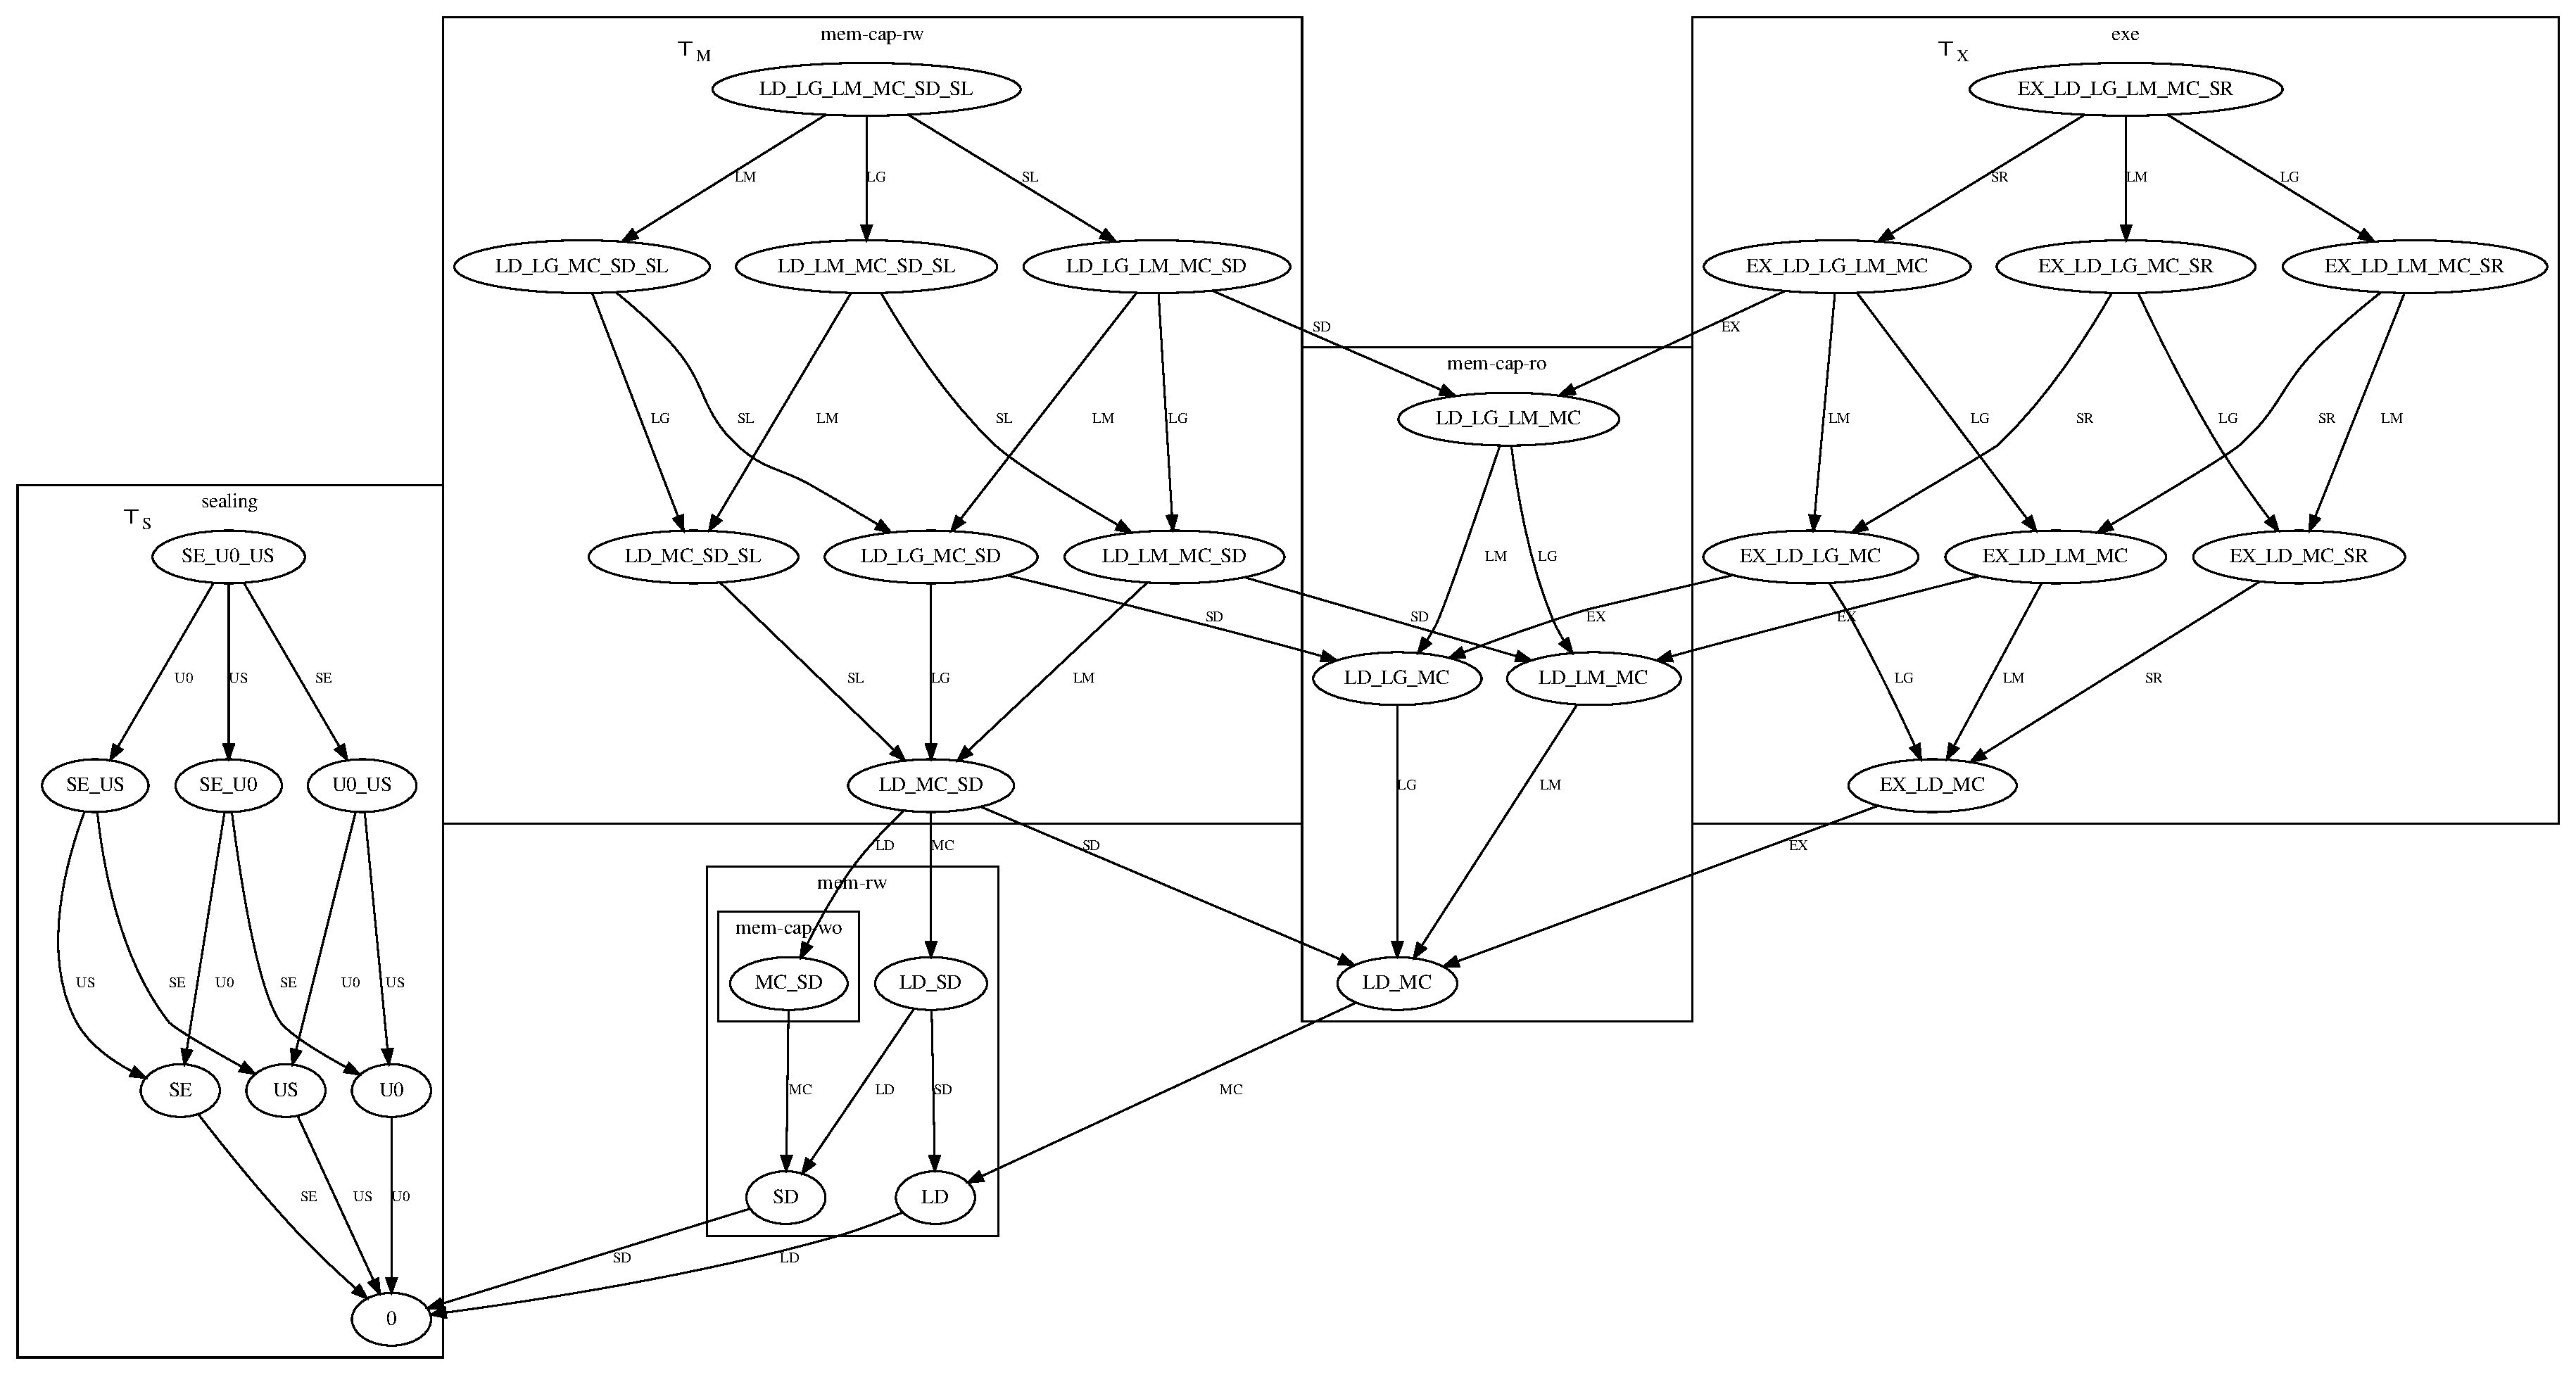
\includegraphics[width=\hsize]{misc/perms/perms5_clustered.pdf}
        \caption{\label{fig:perms5clustered}Graph of allowed permission combinations, grouped by encoding format and ordered by inclusion.
        Edges are labelled with the permission that is dropped by that transition.
        Edges implied by transitivity are omitted.
        \cappermG is omitted because it is entirely orthogonal.}
    \end{figure}
\end{landscape}
\restoregeometry

\insnriscvref{CAndPerm} operates on the decompressed permissions so it is possible to request combinations that cannot be represented in the compressed encoding (for example \cappermX but not \cappermL).
In that case the resulting capability will have a (possibly empty) subset of the requested permissions.
The following procedure is used to encode a given set of requested permissions:
\begin{enumerate}
\item If the permissions include EX, LD and MC then encode SR, LM and LG using the executable format.
\item Otherwise, if the permissions include LD, MC and SD then encode SL, LM and LG using the cap-read-write format.
\item Otherwise, if the permissions include LD and MC then encode LM and LG using the cap-read-only format.
\item Otherwise, if the permissions include SD and MC then encode using the cap-write-only format.
\item Otherwise, if the permissions include LD \emph{or} SD then encode using the data-only format.
\item Otherwise, encode U0, SE and US using the sealing format.
\end{enumerate}
Any permissions that cannot be encoded using the chosen format are dropped.
The possible clearing of GL and LG or SD and LM during capability loads can be quite easily performed on the compressed format although note that clearing SD may require switching format and that SL may be cleared as a side-effect.

Note that this legalization of permissions must happen at all points where permissions can change (\insnriscvref{CAndPerm} and \insnriscvref{CLC}).
For example, the result of \asm{CAndPerm} followed by \asm{CGetPerm} should be consistent regardless of whether the register file stores the permissions in the compressed or decompressed form.
Similarly, storing then loading a capability should not change the permissions except possibly GL, LG, LM and SD as specified by \insnriscvref{CLC}.


\subsection{Sealed capabilities}
\label{sec:sealing}
The \cotype{} field is used for \emph{sealing} capabilities.
A sealed capability cannot be modified or used as authority for operations except special unsealing ones, but can be passed as a token and later unsealed.
Two kinds of sealing are supported:

\begin{description}
  \item[Using otypes:] \insnriscvref{CSeal} allows the creation of sealed capabilities with a given value of \cotype{} given a capability to seal and an authorizing capability with \cappermSeal and the address set to the desired \cotype{}.
   \insnriscvref{CUnseal} permits unsealing a sealed capability if provided with a capability with \cappermUnseal and bounds that contain the \cotype{} of the capability to be unsealed.
  \item[Sealed entry capabilities (sentries):] Executable capabilities sealed with the special \emph{sentry} \cotype{}s can be used with \insnriscvref{CJALR}.
  The capability is unsealed before jumping to it, creating a form of call gate.
  Three kinds of sentry are defined that affect \asm{mstatus.MIE} in different ways: either leaving it unchanged, enabling interrupts or disabling interrupts.
  Jumping to an interrupt enabling or disabling sentry will set or clear \asm{mstatus.MIE} accordingly.
  Additionally, if the link register is \asm{\$cra}, the capability stored by \insnriscvref{CJAL} and \insnriscvref{CJALR} is sealed as a sentry with the current interrupt status: if MIE is set it will produce an interrupt enabling sentry and if it is cleared it will produce an interrupt disabling sentry.
\end{description}
The \cotype{} field uses the following values:
\begin{description}
  \item[0] unsealed
  \item[1] sealed as interrupt inheriting forward sentry
  \item[2] sealed as interrupt disabling forward sentry
  \item[3] sealed as interrupt enabling forward sentry
  \item[4] sealed as interrupt disabling backward sentry
  \item[5] sealed as interrupt enabling backward sentry
  \item[6-7] executable capability sealed with given \cotype{}
  \item[8] reserved (due to encoding)
  \item[9-15] non-executable capability sealed with given \cotype{}
\end{description}
The \cotype{}s $1-7$ can only be applied to executable capabilities, while memory and sealing format capabilities can only be sealed with \cotype{}s $9-15$.
If the \cotype{} field of a memory or sealing format capability is non-zero then bit 3 is implicitly set i.e. \cotype{}s $9-15$ are encoded using values $1-7$.
An attempt to use \insnriscvref{CSeal} or \insnriscvref{CUnseal} with a reserved \cotype{}, or with an \cotype{} not applicable to the capability format, will clear the capability tag.

Because CHERIoT allows manipulating the status of the interrupt through a function call (and function return) by encoding the interrupt type in the otype, the following attack can occur: A caller calling an interrupt-disabling callee can set the return sentry of the callee to the same callee. This means, the callee will call itself on return all the while operating with interrupts disabled. This will lead to infinite repeated calls to the callee with interrupts disabled, violating availability. This attack can be prevented in CHERIoT by adding two new ``backwards-edge'' sentries and adding more checks on \insnriscvref{CJALR}, i.e. only the following combinations are allowed in \insnriscvref{CJALR}:

\begin{center}
  \footnotesize
  \begin{tabular}{|c|c|c|c|}
    \hline
    \asm{cs1} & \asm{cd} & Used for & Valid \asm{cs1} \cotype{}s \\
    \hline
    \asm{\$cra} & \asm{\$cnull} & Function return & Backward sentries $(4, 5)$\\
    $\ne$ \asm{\$cra} & \asm{\$cnull} & Tail call & Unsealed or IRQ inheriting forward sentry $(0, 1)$\\
    any & $\not\in \{ \text{\asm{\$cnull}}, \text{\asm{\$cra}} \}$ & Code outlining & Unsealed or IRQ inheriting forward sentry $(0, 1)$\\
    any & \asm{\$cra} & Function call & Unsealed or forward sentries $(0, 1, 2, 3)$\\
    \hline
  \end{tabular}
\end{center}

\noindent Both \insnriscvref{CJAL} and \insnriscvref{CJALR} with non-\asm{\$cnull} \asm{cd} operands
determine the \cotype{} of the generated capability as a function of the \asm{cd} target itself:

\begin{center}
  \footnotesize
  \begin{tabular}{|c|c|}
    \hline
    \asm{cd} & Generated \asm{cd} \cotype{} \\
    \hline
    $\not\in \{ \text{\asm{\$cnull}}, \text{\asm{\$cra}} \}$ & 0 (unsealed) \\
    \asm{\$cra} & 4, 5 (backward sentries, caller's IRQ disposition) \\
    \hline
  \end{tabular}
\end{center}

Thus, ordinary function calls, for which the calling convention is to use \asm{\$cra} as the return register,
can call any unsealed (executable) capability or forward sentry,
and will always create backward sentries, suitable for the function return case.
Tail calls, which must preserve \asm{\$cra} for their callee and do not generate return capabilities of their own,
are also permitted.
Last, code \emph{outlining}, the dual of code \emph{inlining}, is supported;
outlined code may use a specialized calling convention, not using \asm{\$cra} to exit
(so return from such outlined code looks like a ``tail call'' in the above table),
especially in cases where the outlined code must preserve \asm{\$cra} for its caller.
In this case, the \insnriscvref{CJAL} or \insnriscvref{CJALR} used to enter the outlined code
will have a \asm{cd} that is neither \asm{\$cnull} nor \asm{\$cra},
and so will create \emph{unsealed} return capabilities,
so that all forward sentries in the system must have been built by the RTOS loader.
(Outlined code that \emph{does} use \asm{\$cra} as its return address will also function correctly,
as if it were an ordinary function call and return.)

Given the overloading of the single \insnriscvref{CJALR} instruction,
with register selector operands selecting between multiple semantics,
compilers \emph{must} be careful to use matching entry and exit \insnriscvref{CJALR}s.
For example, entering a function with a \asm{\$cra} link register,
transfering the contents of \asm{\$cra} to another register,
and then ``tail calling'' through that latter register will not work on CHERIoT,
even though analogous code would have worked on base RISC-V.

\subsection{Capability bounds}
\label{sec:bounds}

The capability bounds (\cbase{} and \ctop{}) are stored in a compressed format relative to the \caddress{}, similar to CHERI Concentrate~\cite{Woodruff2019}.
The floating point encoding stores $2^e$-aligned bounds, where $e$ is the exponent.
An exponent of zero can express bounds with byte precision but limits the maximum length of the range to 511 bytes.
Larger exponent values can represent larger ranges, but require more aligned bounds.

To form the \cbase{} and \ctop{} the 9-bit $B$ and $T$ fields from the encoding are inserted into the address at bit $e$ as follows:

\begin{center}
% spread out the table a bit otherwise it is too tight for maths
{
\renewcommand{\arraystretch}{1.5}
\begin{tabular}{r|c|c|c|}
\cline{2-4}
address, $a =$ & $a_\text{top} = a[31:e+9]$ & $a_\text{mid} = a[e+8:e]$  & $a_\text{low} = a[e-1:0]$ \\ \cline{2-4}
base, $b =$    & $a_\text{top}+c_\text{b}$   & $B $ & $0$ \\ \cline{2-4}
top, $t =$     & $a_\text{top}+c_\text{t}$   & $T $ & $0$ \\ \cline{2-4}
\end{tabular}
}
\end{center}

Where the top bits of the address are `corrected' according to the following formulae:

\begin{center}
\begin{tabular}{r c l p{1em} r c l}
$c_b$ & = & $\begin{cases}
-1, & \text{if } a_\text{mid} < B \\
0,  & \text{otherwise}
\end{cases}$ 
&&
$c_t$ & = & $\begin{cases}
  -1, & \text{if } a_\text{mid} < B \text{ and } T \ge B \\
  1,  & \text{if } a_\text{mid} \ge B \text{ and } T < B \\
  0,  & \text{otherwise}
\end{cases}$
\end{tabular}
\end{center}

These corrections ensure that the decoded bounds remain the same provided the address is in $[b, b + 2^{e+9})$, the so-called \emph{representable range}.
They work by testing for conditions that indicate whether the \ctop{} and \caddress{} are in the same $2^{e+9}$ aligned region as \cbase{}.
The representable range spans two such regions (one if $B = 0$), which we will call the lower and upper regions, with $b$ always lying in the lower region.
The ISA is constructed to ensure that, for valid capabilities, $a$ and $t$ are in the representable range and $b \le t$.
Therefore if $a_{mid} \lt B$ then $a$ must be in the upper region, where the $a_{top}$ bits are one greater than those bits in $b$.
Similarly if $T \lt B$ then $t$ must lie in the upper region and we can compute the necessary correction based on whether $a$ also lies in the upper region.
To maintain the necessary invariant for this to work \insnriscvref{CSetAddr} and \insnriscvref{CIncAddr} clear the \ctag{} if the \caddress{} to goes outside the representable range (see \cref{sec:repcheck}).

In order to permit the format to represent a range covering the entire address space using only a 4-bit exponent there is a special case when $E$ has its maximum value.
The effective exponent, $e$, is defined as:

\begin{center}
\begin{tabular}{r c l}
$e$ &=& $ \begin{cases}
              24,& \text{if } E = 15 \\
              E,& \text{otherwise}
\end{cases} $ \\
\end{tabular}
\end{center}

Thus the root memory capability has $B =$ 0, $T =$ 0x100, $E = 15$ and decodes to the range $[0,2^{32})$.
Note that the decoded top is actually a 33-bit value to accommodate this.

\begin{table}
  \centering
  \begin{tabular}{lrr}
  \toprule
  e  &  alignment, $2^e$ &  maximum length, $511 \times 2^e$ \\
  \midrule
  0  &          1 &         511 \\
  1  &          2 &        1,022 \\
  2  &          4 &        2,044 \\
  3  &          8 &        4,088 \\
  4  &         16 &        8,176 \\
  5  &         32 &       16,352 \\
  6  &         64 &       32,704 \\
  7  &        128 &       65,408 \\
  8  &        256 &      130,816 \\
  9  &        512 &      261,632 \\
  10 &       1,024 &      523,264 \\
  11 &       2,048 &     1,046,528 \\
  12 &       4,096 &     2,093,056 \\
  13 &       8,192 &     4,186,112 \\
  14 &      16,384 &     8,372,224 \\
  24 &   16,777,216 &  8,573,157,376 \\
  \bottomrule
  \end{tabular}
  \caption{\label{tab:caplen}
  Capability bounds alignment and maximum length by exponent value.
  Note that for $e=24$ the maximum length exceeds the size of the address space.
  The length of the root capabilities is $2^{32} = 4,294,967,296$ so no valid capability will ever exceed this length.
  }
\end{table}

\subsection{Set bounds operation}
The \insnriscvref{CSetBounds} instruction must select values for $E$, $B$, and $T$ that encode a requested range defined by a given base, $b$, and length, $l$.
In the case that the requested range is not precisely representable \cbase{} is rounded down and \ctop{} up to multiples of $2^e$, where $e$ is the chosen exponent.
For maximum bounds precision, we desire the smallest $e$ that can represent the requested region.
From the encoding we can observe that the largest encodable length for a given $e$ is given by $2^e \times (2^9 - 1)$.
Therefore we require a solution to the inequality:
\[
\begin{array}{r c l l}
l & \le & 2^e \times (2^9 - 1)\\
l & \le & 2^{e+9} - 2^e\\
l & \le & 2^{e+9} & \text{approximation}\\
\log_2 l & \le & e+9 \\
\lfloor \log_2 l \rfloor & \le & e + 9 & \text{approximation} \\
\msb(l) & \le & e + 9 & \text{index of most significant set bit is floor of } \log_2 \\
32 - \clz(l) & \le & e + 9 & \text{also expressible as count leading zeros for 32-bit length} \\
23 - \clz(l) & \le & e \\
e & = & 23 - \clz(l) & \text{since we require the smallest e} \\
\end{array}
\]
Since $e$ must be greater than or equal to zero the count leading zeros should be limited to the top 23 bits of $l$ (lengths smaller than 9-bits are expressed with $e = 0$).
% To ensure there is some representable buffer and to accommodate rounding we increment the chosen exponent by one if the length is close to the maximum representable:
% \[
% e' =
% \begin{cases}
% e + 1,\text{ if }l[e+8:e+1] = \text{\asm{0xff}} \\
% e,\text{ otherwise}
% \end{cases}
% \]
Since the exponent is limited to 4-bits, exponents greater than 14 are mapped to the special maximum exponent, 24, which is encoded as 15:
\[
e'=
\begin{cases}
  e,\text{ if } e \le 14 \\
  24,\text{ otherwise}
\end{cases}
\]
Having chosen the exponent, the relevant bits of \cbase{} and \ctop{}, $t = b + l$, are extracted:
\[
  B = b[e' + 9: e'] \hspace{2em} T = t[e' + 9: e']
\]
The bounds are exact if the bits below $e'$ in both $b$ and $t$ are all zero.
By discarding the lower bits of $b$ the \cbase{} is automatically rounded down to a representable value,
but if the top is not exact then we must round it up by incrementing by one to ensure the encoded range includes the requested top.
Note that the calculated $e'$ was based on the requested length, but having rounded the bounds the resulting length may be larger and may exceed the maximum representable length for $e'$.
To check for this we calculate the encoded length $T - B$ (in units of $2^e$), and compare it with the maximum encodable length, $2^9 - 1$.
Note that $B$ and $T$ above are one bit wider than the encoding can store for this purpose.
If the maximum encodable length is exceeded we increment $e$ by one and recompute $B$ and $T$, this time with a guarantee that the resulting length is encodable.
Finally, the oversized $B$ and $T$ can drop their extra most significant bit in the final encoding.
\subsection{Representability checks}
\label{sec:repcheck}

To enable capabilities to be used to implement pointers in the C language the capability encoding is designed to allow the \caddress{} to vary within a limited range without changing the decoded bounds.
The \emph{representable range} of a capability is the set of addresses for which the decoded bounds remain the same.
We also wish to maintain the \emph{monotonicity} invariant that the bounds of a valid capability must be a subset of the bounds of the valid capability from which it is derived.
Therefore, whenever the \caddress{} of a capability changes the hardware must check whether the new address remains within the representable range, otherwise the new bounds would violate this invariant.
For example, if \insnriscvref{CSetAddr} or \insnriscvref{CIncAddr} detects that the new \caddress{} is outside of the representable range then the \ctag{} of the result is cleared.

The representation guarantees that the bounds remain decodable provided the address, $a$, and base, $b$, satisfy $b \le a$ and $a \lt b + 2^{e+9}$.
Additionally, if $e$ is 24 then all addresses are representable.
The representable range always includes \ctop{}, although in some cases it is the highest representable address.
Therefore the representation meets the C-language requirement that pointers may range within object bounds or `one byte past the end'.
Other CHERI implementations include much larger representable ranges than this minimum in order to accommodate common C programming practices.
However, this comes at the cost of bits in the representation and our experience so far has shown that it is not necessary for embedded systems.

The following instructions all set the capability \caddress{} and therefore require a representability check:
\begin{itemize}
  \item \insnriscvref{AUIPCC}
  \item \insnriscvref{AUICGP}
  \item \insnriscvref{CSetAddr}
  \item \insnriscvref{CIncAddr}
\end{itemize}
Note that although \insnriscvref{CJAL} and \insnriscvref{CJALR} also set the address on the link register, it is guaranteed to be representable because its \caddress{} can be at most equal to \PCC{}.\ctop{} given that the jump itself is in bounds.
Therefore no representability check is required for these instructions.

Bounds exceptions on instruction fetch might result in an unrepresentable \MEPCC{}.
To simplify hardware while preserving capability monotonicity the tag of \MEPCC{} is always cleared on instruction fetch bounds violations.
This unrepresentability might mean that the decoded bounds of \MEPCC{} do not match the bounds of \PCC{} at the time of the exception,
but \MEPCC{}.\caddress{} will contain the address of the faulting instruction or instruction fetch.

Validation of \MTCC{} and \MEPCC{} in \insnriscvref{CSpecialRW} prevents potential unrepresentability due to the legalisation of \asm{mtvec} and \asm{mepc}.
To simplify hardware these special registers are validated on write, with violations clearing the tag of the value stored (\cref{sec:scrs}).

\subsection{The NULL capability}
\label{sec:null}

The NULL capability is defined as an untagged capability with an \caddress{} of zero and an encoding of all zeroes.
This definition is for maximum compatibility with the C language, where it is used to represent NULL pointers.
The NULL capability is also used as the value of the \asm{\$c0} register and to store integer results by setting the \caddress{} to the required value.
Although capability fields other than the \caddress{} are not meaningful on untagged capabilities they may be queried using the \asm{CGetX} instructions.
Thus it can be observed that the NULL capability decodes as an untagged, unsealed capability, with no permissions, \cbase{} $0$ and \clength{} $0$\footnote{
  On other CHERI architectures the NULL capability is defined to have maximum length.
  This could be achieved by tweaking the encoding (e.g. by inverting the encoded exponent and making the zero value a special case), but there is no clear advantage to doing this.
}.
Note that NULL-derived capabilities with a non-zero address may have non-zero \cbase{} and \ctop{}, but will be untagged.

\subsection{Zero length capabilities}
\label{sec:zerolengthcaps}

The capability encoding described supports capabilities with zero length, where \cbase{} is equal to \ctop{}.
Such capabilities do not authorize access to any memory (or sealing rights), so it may be tempting to use them as unforgeable tokens (e.g. to implement file handles), however they come with a big drawback:
zero length capabilities can be derived with \cbase{} equal to the \ctop{} of an existing capability, even though that capability does not authorize access to \ctop{}.
To give an example of this suppose a memory allocator gives out two capabilities with adjacent ranges $[a,b)$ and $[b,c)$.
Later it may receive a call to `free' with a zero length capability $[b,b)$ and it has no way to tell which of the two ranges it was derived from.
If it relies only on the \cbase{} of the capability and does not validate the length the allocator may incorrectly free $[b,c)$.
The same problem arises during revocation sweeps as performed by Cornucopia~\cite{cornucopia}, meaning it is unable to revoke zero length capabilities.
Therefore we strongly discourage the use of zero length capabilities and encourage validating the length of untrusted capabilities.
As an alternative we suggest using capabilities of length one derived from the sealing root but without \cappermSeal or \cappermUnseal.
In this case \cappermUZ may be used as a software defined permission.

\TODO{Consider having CSetBounds clear the tag on zero length caps to avoid these problems. This would also be necessary if we moved to an encoding that doesn't allow zero length caps.}

\subsection{Zero permission capabilities}

In a similar vein to zero length capabilities the encoding also supports capabilities with no permissions.
These are encoded using the sealing format but may be derived from any of the roots.
We therefore caution against using zero permission capabilities as tokens, because the ability to derive the same capability from either a memory or a sealing root may break the expected unforgeability property.
They may also behave unexpectedly with respect to revocation, since sealing capabilities are not subject to revocation but memory capabilities are.
Given these limitations it is not clear that zero permission capabilities should be allowed at all and support may be removed in future revisions.

\subsection{Capability layout in memory}

While \cref{fig:capformat} shows the nominal capability format, for microarchitectural reasons it may be preferable for the capability fields to appear in a different arrangement in memory.
Future versions of the architecture may also specify a different capability format.
Therefore software should not rely on the exact layout of capabilities in memory.
This said, we expect that certain software will need knowledge of the capability format.
For example, memory allocators and the toolchain will need to be aware of alignment requirements and a debugger will need to be able to decode capabilities from memory dumps.

\subsection{Sail implementation}

\cref{chap:sailenc} contains Sail code implementing the capability
encoding described here as well as properties validated using SMT.

\section{Instruction compression}
\label{sec:c-extension}

Compressed load and store extensions from the standard RV32 C extension decompress to their capability equivalents.
Similar to the encodings of \insnriscvref{CLC} and \insnriscvref{CSC} in uncompressed instructions, the C extension uses compressed \asm{C.LD} and \asm{C.SD} from RV64 to encode \insnriscvref{CLC} and \insnriscvref{CSC}.
In RV32 these opcodes are used to encode \asm{C.FLW} and \asm{C.FSW}, meaning these compressed encodings for floating point loads and stores are no longer available.
Note that this applies to C instructions with implicit stack operands, that is we use \asm{C.LDSP} (RV64) and \asm{C.SDSP} (RV64) as capability loads and stores relative to the stack capability, replacing the \asm{C.FLWSP} (RV32) and \asm{C.FSWSP} (RV32) encodings.
Such a decision is justified because capability loads and stores greatly outnumber floating point instructions in embedded code, and most devices this ISA is targeting do not have a floating point unit at all.

Implicit stack pointer arithmetic instructions are not useful with CHERI, as adding an offset with \asm{ADD} will produce an untagged integer.
These instructions are modified to decode to \insnriscvref{CIncAddr} to produce valid stack-derived capabilities.
As a result, \asm{C.ADDI16SP imm} is decoded into \asm{CIncAddr \$csp, \$csp, imm} and \asm{C.ADDI4SPN \$rd, imm} into \asm{CIncAddr \$cd, \$csp, imm}.

The \cherimcuisa{} introduces changes to mappings between certain compressed and uncompressed instructions, but no changes to the encodings of compressed instructions themselves.
This translates to minimum logic modifications when adding \cherimcuisa{} support to an existing RISC-V CPU.
However, experiments in \cref{chap:c-changes} show that further code size reduction can be achieved by introducing changes in the encoding themselves, to accommodate RV32E and CHERI instructions.

\section{Stack high water mark}
\label{sec:shwm}

The stack high water mark is a simple mechanism in \cherimcu{} to track stack use so that the RTOS switcher implementation can minimise the amount of stack zeroing during compartment calls.
The mechanism uses two new integer CSRs: the stack high water mark, \mshwm{} (\asm{0xBC1}), and the stack high water mark base, \mshwmb{} (\asm{0xBC2}).
These may be read and written using the \asm{CSRRW} instruction only if \PCC{} has \cappermASR{}, otherwise an attempt to do so will result in a Reserved Instruction exception.
The four least significant bits of both registers are hardwired to zeros, making them 16-byte aligned.
Any write with these bits set is legalised by rounding down.

On every memory write the address of the write (the lowest byte written) is compared to \mshwm{} and \mshwmb{}.
If the address is greater than or equal to \mshwmb{} and less than \mshwm{} then \mshwm{} is updated with the address of the write (rounded down to 16-byte alignment).
Thus, if \mshwmb{} is set to the stack base (the lowest stack address) and \mshwm{} is initialised to the top of the stack, then \mshwm{} will track the lowest stack address written during execution.
Since stacks grow downwards this indicates the maximum stack usage.
The RTOS uses this to optimise stack zeroing by maintaining an invariant that the stack between \mshwmb{} and \mshwm{} for each thread is always zeroed.
The stack high water mark CSRs are saved and restored during context switches along with other thread state.

Note that only the address of the store is accounted for, not the width.
This means that it is possible for an unaligned store with an address below \mshwmb{} to write bytes above \mshwmb{} without updating \mshwm{}.
For example, a 4-byte store to \mshwmb{}$ - 1$ would write the bytes at \mshwmb{}$\dots{}$\mshwmb$+ 2$ but leave \mshwm{} unchanged, potentially breaking the RTOS's invariant.
In practice this is not a problem as the RTOS will never issue a capability to untrusted code that crosses the stack base and would therefore permit such a write.%
\footnote{In fact, no such capabilities should exist after the loader has run and initialised the thread data structures.}
Given this, we choose not to unnecessarily complicate the hardware by requiring it to handle this corner case.
